\chapter{Implementaci\'on y Resultados}
\label{cap:implementacion}

%%%%%%%%%%%%%% CASO 1
\section{Dataset: Covid-19}
\label{intro:covid}

\subsection{Implementaci\'on}

\begin{lstlisting}[language=python]
total_train = sum(len(files) for _, _, files in os.walk(traindir))
pbar = tqdm(total=total_train, desc='Loading training images')
for d in os.listdir(traindir):
    categories.append(d)
    train_imgs = os.listdir(os.path.join(traindir, d))
    valid_imgs = os.listdir(os.path.join(validdir, d))
    test_imgs = os.listdir(os.path.join(testdir, d))
    n_train.append(len(train_imgs))
    n_valid.append(len(valid_imgs))
    n_test.append(len(test_imgs))

    for i in train_imgs:
        img_categories.append(d)
        img = cv2.imread(os.path.join(traindir, d, i))
        img_array = np.array(img)
        pbar.update(1)
        hs.append(img_array.shape[0])
        ws.append(img_array.shape[1])
pbar.close()

cat_df = pd.DataFrame({'category': categories,
                       'n_train': n_train,
                       'n_valid': n_valid,
                       'n_test': n_test}).\
                        sort_values('category')

cat_df.sort_values('n_train', ascending=False, inplace=True)
\end{lstlisting}

\vspace*{0.5cm}

%%%%%%%%%%%%%%%%%% CASO 2
\clearpage
\section{Reconocimiento Facial} % 
\label{intro:face_detector}

\subsection{Implementaci\'on}

\begin{center}
  \begin{tikzpicture}[node distance=2cm]
    \node (node0) [startstop] {Conjunto de im\'agenes};
    \node (node1) [process, right of=node0, xshift=4cm] {Detecci\'on Facial};
    \node (node2) [process, below of=node1] {Alineaci\'on Facial};
    \node (node3) [process, below of=node2] {Extraer Incrustaciones};
    \node (node4) [fit, below of=node3] {Fitear un SVM con las incrustaciones};
    \node (node5) [startstop, below of=node4] {Reconocimiento facial en im\'agenes y v\'ideos};
    
    \draw [arrow] (node4) --node[anchor=east] {\small{guardar modelo}} (node5);
    \draw [arrow] (node3) --node[anchor=east] {\small{128-d OpenFace}} (node4);
    \draw [arrow] (node2) --node[anchor=east] {\small{68 hitos con DLIB}} (node3);
    \draw [arrow] (node1) --node[anchor=east] {\small{recortar caras}} (node2);
    \draw [arrow] (node0) --node[anchor=south, text width=3.5cm, align=center] {\small{caffemodel}} (node1);
  \end{tikzpicture}
 \vspace*{0.5cm}
\captionof{figure}[Diagrama de flujo detecci\'on facial]{Diagrama de Flujo en la implementaci\'on para el reconocimiento y clasificaci\'on facial}
\label{fig:flowface}
\end{center}

\vspace*{0.5cm}

%%%%%%%%%%%% CASO 3
\clearpage
\section{YOLO: Detector de Mascarillas}  % yolo
\label{imple:yolov5}

\subsection{Implementación}

\subsection{Resultados}
\label{imple:yoloResults}


\begin{figure}[htb]
    \centering % <-- added
\begin{subfigure}{0.45\textwidth}
  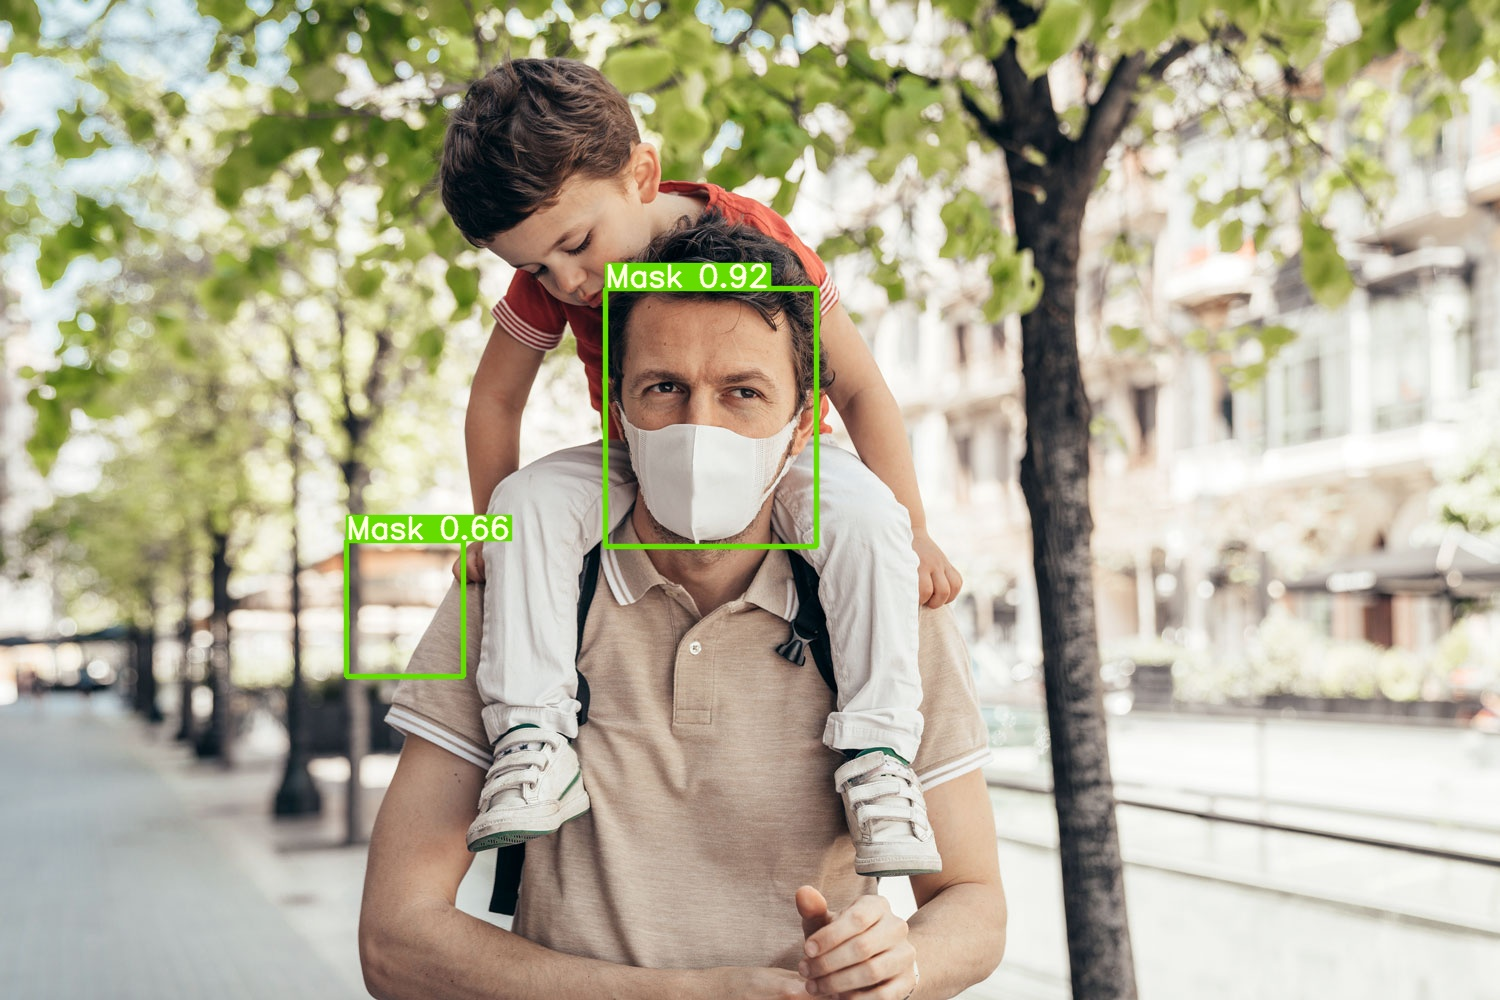
\includegraphics[width=\linewidth]{images/covid_test5.jpg}
  \caption{Hay una sobredetección de un rostro con mascarilla y una baja detección de un rostro sin mascarilla.}
  \label{fig:1}
\end{subfigure}\hfil % <-- added
\begin{subfigure}{0.45\textwidth}
  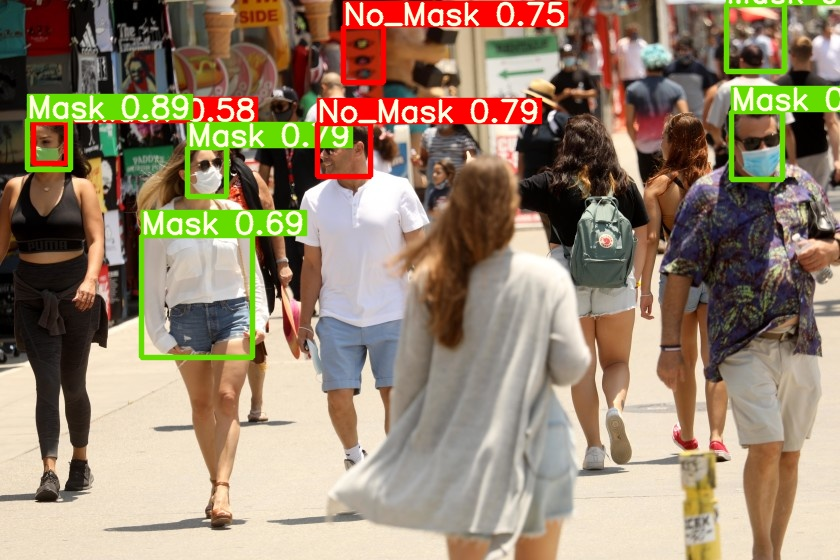
\includegraphics[width=\linewidth]{images/covid_test2.jpg}
  \caption{Hay una sobredetección, No-Mask, sobre una detección correcta, esto se podría corregir con un umbral mayor de Non-maximum Suppression.}
  \label{fig:2}
\end{subfigure}\hfil % <-- added

\medskip
\begin{subfigure}{0.45\textwidth}
  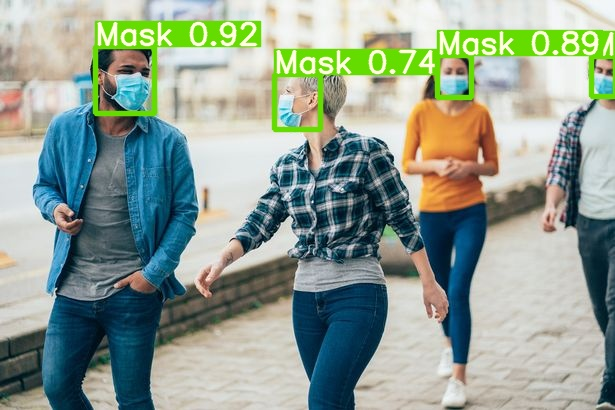
\includegraphics[width=\linewidth]{images/covid_test6.jpg}
  \caption{Todas las personas usando mascarillas se han detectado correctamente.}
  \label{fig:4}
\end{subfigure}\hfil % <-- added
\begin{subfigure}{0.45\textwidth}
  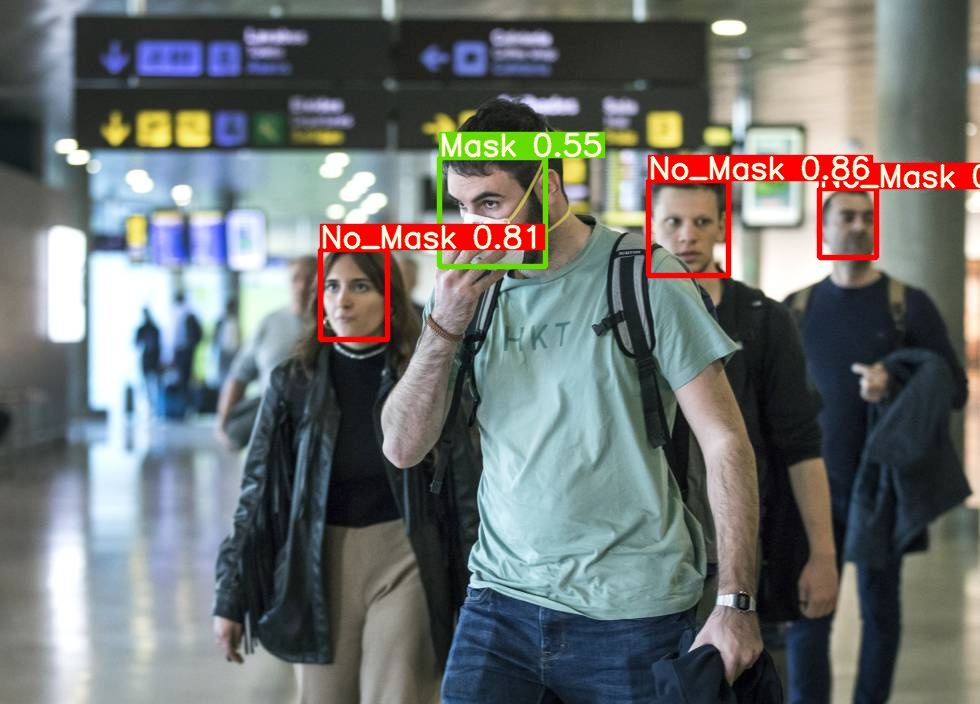
\includegraphics[width=\linewidth]{images/covid_test8.jpg}
  \caption{Se he detectado correctamente las personas con y sin mascarillas.}
  \label{fig:5}
\end{subfigure}\hfil % <-- added
\caption[Imágenes de pruebas]{Imágenes reservadas para pruebas. Aunque las métricas del modelo son bastante favorables, en producción, el modelo podría tener un error mucho más alto. La única manera de corregirlo es aumentar la cantidad de datos de entrenamiento recopilando más imágenes y anotaciones.}
\label{fig:yolotests}
\end{figure}